\documentclass[12pt]{article}

\oddsidemargin=-.25in
\evensidemargin=-.25in
\textwidth=7in
\topmargin=-.5in
\textheight=9in
\parindent=0in

\usepackage[english]{babel}
\usepackage[utf8x]{inputenc}
\usepackage{amsmath}
\usepackage{graphicx}
\usepackage[colorinlistoftodos]{todonotes}

\title{Using Linear Models to find Value in \\Major League Baseball Players}
\author{Michael Scarinci \\MATG 611 \\Computational Methods for Analytics}

\begin{document}
\maketitle

\begin{abstract}
For years, major league baseball clubs and fans have used traditional stats like batting average and on base percentage to evaluate players. The introduction of sabermetrics has created a plethora of new stats to evaluate players. With the use of these measures, players can be evaluated with more accuracy. Baseball is a high variance sport with luck involved. A player can have an unlucky year or be on an ineficent team. This may make the player appear to be underperforming. By using linear regression models we can find these underperforming players and use a buy low approach to get the most value and performance for a club's money. Using this model, we compared Joey Votto, Nelson Cruz and Joc Pederson, and found Nelson Cruz to be a great value player and rookie Joc Pederson to be worth \$8 million. With salaries breaking record highs each season, these techniques are vital for smaller market clubs to compete with the large market clubs.
\end{abstract}

\section{An Introduction to the World of Baseball}

\subsection{Baseball's Salaries and Club Expenditures}
\qquad Baseball is constantly referenced as America's Pastime. With a 162 game regular season there are plenty of opportunities for a fan to get out and watch a game. Due to the long regular season, the players of the game demand high salaries. The average major league baseball player made \$4.25 million for the 2015 regular season. Major League Baseball does not have a salary cap, therefore team owners with the most money can buy out the free agent pool to acquire the best talent. The Los Angeles Dodgers ranked highest in payroll for 2015 spending over \$272 Million for 2015. Opposite the Dodgers were the Miami Marlins who spent just over \$68 Million for the 2015 season. The Kansis City Royals, who won the 2015 World Series, were ranked in the middle of the pack while spending over \$113 Million \cite{deadspin}. For the smaller market teams, it is vital to find value in players who may appear to have underperformed.


\subsection{Statistics Used}
\qquad To find value in players, we must understand important statistics used in creation of the model \cite{fangraphs}.
 \begin{description}
  \item[$\bullet$ Batting Average(AVG)] - the ratio of a batter's hits per at bat, excluding walks and hit by pitches.
  \item[$\bullet$ On Base Percentage(OBP)]  - Measures how often a batter reaches base, including walks and hit by pitches. 
  \item[$\bullet$ wOBA]  - Weighted on Base Average attempts to give weight to the type of hit. A double is weighted heavier than a single, while a triple is weighted higher than a double.
  \item[$\bullet$ ISO]  - A measure of a hitter's power, slugging percentage minus batting average
  \item[$\bullet$ WAR]  - Wins Above Replacement gives a value to a player based on the average performance, a very complicated measure that is constantly being changed.
  \item[$\bullet$ wRC]  - Weighted Runs Created gives a percentage of the runs created by a hitter versus the league average. The league average is at 100, for every point higher or lower is a percentage point. 
\end{description}

\subsection{Measuring Player effectiveness}
\qquad To evaluate players I used runs accounted per plate appearance(RAPA):
\begin{center}
$RAPA = \frac{Runs + RBI's - HR's}{Plate Appearances}$
\end{center}
In order to avoid duplication of runs, the hitter's home runs were subtracted. The ratio of Runs Accounter per Plate appearance was to avoid bias in players who faced injuries. It also avoided non-everyday players. Runs accounted was used due to runs being vital for a team to win games. The objective of any game is to score more runs than the other team. Runs accounted is a direct measure of the value a player brings to a team.

\section{Data Collection and Manipulation}

\subsection{Collecting Data}


\qquad All player data and team data was collected from Fangraphs.com. They collect all player statistics for every season. The player data consisted of 143 players from the 2015 season with a minimum of 500 plate appearances\cite{fangraphs}. Fangraphs also has the statistics for each team, for every season. All data was exported in .csv file extensions and imported to R for manipulation.


\subsection{Manipulating the Data}

\qquad There was not a large need for data manipulation, as the data was already well displayed. Runs accounted per plate appearance had to be calculated for each player, and then added to the data frame. This information was then used to visual the data and make initial observations.


\section{Initial Observations}

\qquad The first steps in analysis was plotting wOBA againt RAPA(Figure 1), and then batting average against RAPA(Figure 2). It appeared that both showed a linear relationship, but batting average showed higher variance. The initial reaction was that wOBA was a better indicator of RAPA. Seeing the outliers as displayed in Figure 2, circled in red, gave me insight into finding possible value players. The value players were Joey Votto, Cincinatti Reds, Nelson Cruz, Seattle Mariners, and Joc Pederson, Los Angeles Dodgers. 

\begin{figure}[h]
\centering
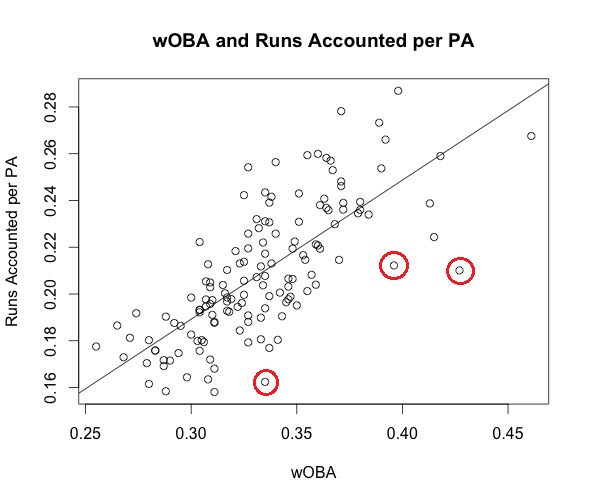
\includegraphics[width=4.5in]{wOBA.png}
\caption{wOBA visual}
\end{figure}

\begin{figure}[h]
\centering
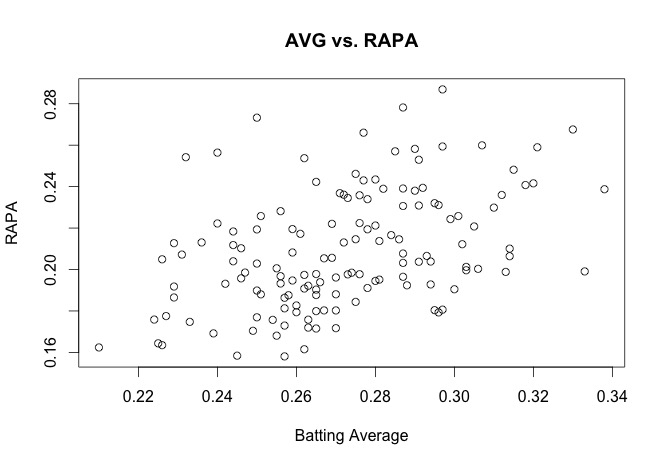
\includegraphics[width=4.5in]{Average.jpeg}
\caption{Batting Average visual}
\end{figure}
 
\subsection{Initial Models}

\qquad While the visual gave insight that wOBA was a better indicator, I created a linear model of both wOBA and batting average with RAPA. The $R^2$ of the wOBA model was .5406, and the $R^2$ of the batting average model was .1839. My initial reaction was correct that wOBA was a better indicator of RAPA. 

\subsection{Finding the Best Statistic for Univariate Regression}
\qquad The next step was to decide which of the six chosen stats was best. Creation and analysis of the model lead me to conclude that wOBA was the best indicator of RAPA, while wRC was second, and batting average was ranked last(Figure 3). From here there were three outliers well below the fit line. These players could be seen as underperforming players that are being undervalued and should be performing better.  

\begin{figure}[h]
\centering
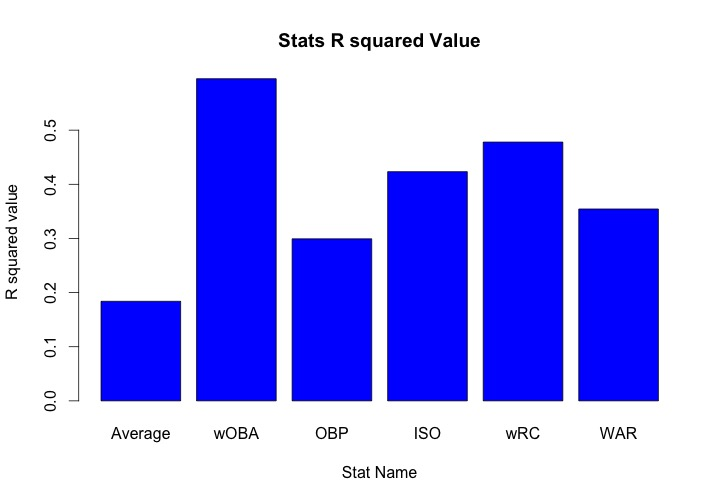
\includegraphics[width=4.5in]{Rsquared.jpeg}
\caption{$R^2$ of each statistic}
\end{figure}


\section{Multivariate Regression}
\qquad The next step was finding the ideal variables for multivariate regression. The addition of any variable to a model, will increase the $R^2$. This will lead to overfitting of data and is not a viable measure for multivariate regression. Using all six variables would not be the guaranteed best fit for the data. Instead, adjusted $R^2$ was used to measure effectiveness.

\subsection{Leaps and regsubfit function}
The leaps package was vital in deciding the best combination of statistics for each count of variable. Using the regsubfit function of the library leaps\cite{stats}, I found the right combination of statistics to use for one variable, two variable, all the up to six variables. The function tests each combination of variables and gives output of the best combination of variables for each count of variable. To pick the ideal number of variables and statistic combination, adjusted $R^2$ was used. Using the summary function, the adjusted $R^2$ value for each amount of variables was returned. The same was done with $R^2$, and as expected $R^2$ was monotonically increasing, while adjusted $R^2$ had a max at five variables(Figure 4).

\begin{figure}[h]
\centering
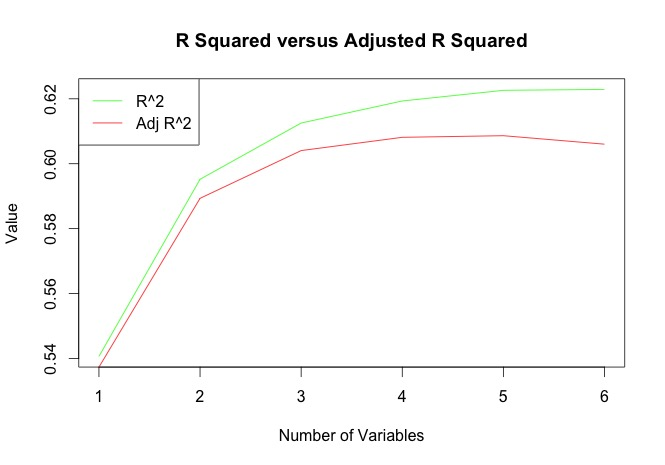
\includegraphics[width=6in]{RvsadjR.jpeg}
\caption{Finding the ideal number of variables using adjusted $R^2$}
\end{figure}

\subsection{Creating the Model}
Using the regsubfit function and the knowledge that five variables gave the best adjusted $R^2$ value, the ideal statistics for a model were found. To create the model, batting average, wOBA, OBP, wRC and WAR were used. Creating the model gave us the equation:
\begin{center}
$\hat{y} = -.082 + (1.551)wOBA + (.095)AVG -(.425)OBP$\\
 $+ (.002)WAR - (.001)wRC$
\end{center}

\section{Results and Conclusion}

\subsection{Results}
\qquad Using the three value players and the model, their fit RAPA was found. Their respective fit values were well above their actual RAPA for the 2015 season. By multiplying their fit RAPA by their plate appearances for the 2015 season, their expcted runs accounted for the 2015 season was found. For all three players their fit runs were significantly higher(Figure 5). While the fit values are not exact, the confidence intervals and prediction intervals were found for the three players(Table 1), which are at a 95\% level.

\begin{figure}[h]
\centering
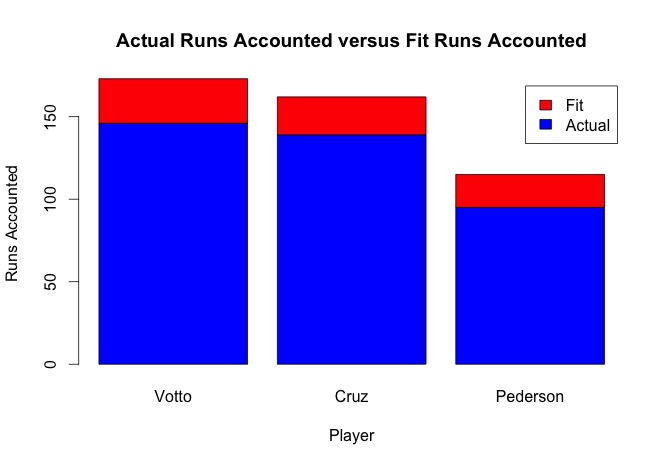
\includegraphics[width=4.5in]{FitRuns.jpeg}
\caption{Fit Runs versus Actual Runs per player}
\end{figure}

\begin{table}[]
\centering
\caption{Fit, Confidence and Prediction Intervals for Three Value Players}
\begin{tabular}{|c|c|c|c|c|c|c|}
\hline
\textbf{Player} & \textbf{Actual} & \textbf{Fit} & \textbf{CI Lower} & \textbf{CI Upper} & \textbf{Prediction Lower} & \textbf{Prediction Upper} \\ \hline
Joey Votto      & .210            & .249         & .236              & .261              & .212                      & .286                      \\ \hline
Nelson Cruz     & .212            & .248         & .239              & .258              & .212                      & .285                      \\ \hline
Joc Pederson    & .162            & .196         & .184              & .208              & .159                      & .233                      \\ \hline
\end{tabular}
\end{table}

\qquad The fit line gives a simlar expected RAPA for Votto and Nelson Cruz (Table 1). Using the information we could conclude that these players are equivalent in run production. Joey Votto's salary for the 2015 season was \$14 Million, while Nelson Cruz was only paid \$8 Million. This offseason a club could have a \$6 Million savings by going after Nelson Cruz rather than Joey Votto. Joc Pederson's value more challenging to predict. He was a rookie for the 2015 season, therefore only making the league minimum of \$500,000. Based on his stats, Pederson still underperformed for the 2015 season based on his statistics. According to the model his RAPA should have been $.196$. Melky Cabrera overperformed in the 2015 season with a .196 RAPA, versus his fit value of $.192$. Pederson's fit RAPA is similar to Cabrera, however Cabrera made \$8 Million for the 2015 season. Using this model can give an idea of value for young players who are still under their rookie contracts.

\subsection{Improvements Going Forward}
\qquad While the model created uses six statistics, it only accounts for batting statistics. Some important factors to take in are fielding stats and how versatile a player is in playing position. Part of this is position scarcity in the market. Depending on the year, there may be a large supply of outfielders which will drive the value down of some players. At the same time first basemen may be in large demand, which will increase the demand for the position, and lead to teams overpaying. An improved model would also account for the player's age. A player is not as productive at thirty eight years old versus thirty years old. 

\qquad Another factor not involved in the model is the player's home ballpark, in which they play 81 games a season. Coor's Field in Colorado is known as Mile High Stadium. The elevation of the stadium has lead to higher run production because of the ball traveling farther. A hitter would overperform in a plus ballpark and his value would not be as high. The same goes for player's whose home ball park is known as a pitcher's ball park. The fences are often farther from home plate in these fields, and would bring down player value. Bringing this factor into the model would give better value to those coming from pitcher ballparks and lower the value of those from hitter friendly ball parks.

\subsection{Conlcusion}
\qquad While the model has some flaws, it is a great start. Bringing in the factors from above would bring an immediate improvement to the model. Moving forward to improve the model, the same tests can be done on data for the 2014 season. As always a larger sample size of data will improve the model. Also to be considered is changing the measure of value from RAPA. RAPA is biased in that a player on a better team will account for more runs. This player will be batting with runners on based more often, therefore creating more oppurtunites to manufacture runs. A less biased measure may be simply reaching base, as this is independent of team performance.



\begin{thebibliography}{1}

\bibitem{fangraphs} Baseball Statistics and Analysis | FanGraphs Baseball. Web. 17 Dec. 2015.

\bibitem{deadspin} Patchesky, Barry. "2015 Payrolls And Salaries For Every MLB Team." Deadspin. N.p., n.d. Web. 17 Dec. 2015.

\bibitem{stats}Dalgaard, Peter. Introductory Statistics with R. New York: Springer, 2002. 

\end{thebibliography}


\end{document}